\documentclass[11pt,a4paper]{article}
\usepackage[margin=22mm]{geometry}
\usepackage{amsmath,amssymb,booktabs,graphicx,array,xcolor}
\usepackage{caption}
\usepackage[hidelinks]{hyperref}
\setlength{\parindent}{0pt}
\setlength{\parskip}{6pt}
\renewcommand{\arraystretch}{1.15}
\captionsetup{font=small,labelfont=bf}
\newcommand{\loss}{\operatorname{Loss}}
\newcommand{\sourcefile}[1]{\texttt{\detokenize{#1}}}
\begin{document}

\begin{center}
{\LARGE\bfseries CSE558: Data Science Assignment}\par
\vspace{4pt}
{\large Random projections on KDD Cup 1999}\par
\vspace{8pt}
Names: \underline{\hspace{43mm}}\quad\underline{\hspace{43mm}}\\[6pt]
Roll numbers: \underline{\hspace{33mm}}\quad\underline{\hspace{33mm}}
\end{center}

\section*{Data preparation}
The default 10\% KDD Cup 1999 dataset was fetched using
\sourcefile{fetch_kddcup99}, with \sourcefile{subset=None} and \sourcefile{as_frame=True}.
The three categorical features (\sourcefile{protocol_type}, \sourcefile{service},
and \sourcefile{flag}) were one-hot encoded, the other 38 features were converted
to floats, and constant columns were removed. Every remaining column was
rescaled to $[0,1]$ using $(x-\min)/(\max-\min)$.
The resulting matrix, stored as \sourcefile{data/D.npy} in float32, has
\[
 D\in\mathbb R^{494021\times116},\qquad n=494021,\quad d=116.
\]
No rows were removed or reordered, so the targets remain aligned with the rows.

\section*{Question 1: JL for $k$-means clustering}
\fbox{\parbox{0.94\linewidth}{\textbf{Placeholder.} Insert the answers, tables,
plots, and discussion for Question 1(a)--(e) here.}}

\section*{Question 2: JL for linear regression}
The target is $y_i=0$ for a normal connection and $y_i=1$ for an attack. We solve
\[
 b=\arg\min_a\loss(D,y,a),\qquad
 \loss(D,y,a)=\|Da-y\|_2^2.
\]
All solves use \sourcefile{numpy.linalg.lstsq} with \sourcefile{rcond=None};
no intercept is added. For CountSketch, each original
row receives an independent uniform bucket and sign in $\{-1,+1\}$.
Signed rows and labels are accumulated directly with \sourcefile{numpy.add.at};
the dense matrix $S$ is never formed for CountSketch.

\subsection*{(a) Full-data baseline}
\begin{center}
\begin{tabular}{lr}
\toprule
Quantity & Result \\
\midrule
Full-data loss $\|Db-y\|_2^2$ & 2949.788815 \\
Time to compute $b$ (seconds) & 2.127519 \\
Numerical rank of $D$ & 113 \\
\bottomrule
\end{tabular}
\end{center}
The timer covers only the least-squares solve. Loading the data and calculating
the loss are excluded. The numerical rank is returned by the same solve;
it is smaller than the number of columns because the columns are not all
linearly independent.

\clearpage
\subsection*{(b) Accuracy after CountSketch}
For each $m$, five fresh sketches were drawn and
$\widetilde a=\arg\min_a\|SDa-Sy\|_2^2$ was computed. Define
\[
 R=\frac{\loss(D,y,\widetilde a)}{\loss(D,y,b)},\qquad
 L_S=\|SD\widetilde a-Sy\|_2^2.
\]
\begin{center}
\small
\begin{tabular}{rrrrrr}
\toprule
$m$ & Mean full loss & Mean $R$ & Min $R$ & Max $R$ & Mean $L_S$ \\
\midrule
50 & 11133.752 & 3.7744 & 3.0140 & 5.6804 & $1.384\times10^{-23}$ \\
100 & 44794.351 & 15.1856 & 6.5828 & 27.8798 & $1.030\times10^{-23}$ \\
200 & 6906.387 & 2.3413 & 1.8277 & 2.7100 & 1274.739 \\
500 & 3821.076 & 1.2954 & 1.2648 & 1.3222 & 2289.017 \\
1000 & 3306.523 & 1.1209 & 1.0948 & 1.1319 & 2624.802 \\
2000 & 3133.200 & 1.0622 & 1.0525 & 1.0764 & 2827.870 \\
5000 & 3017.272 & 1.0229 & 1.0188 & 1.0264 & 2887.240 \\
\bottomrule
\end{tabular}
\captionof{table}{Accuracy over five independent CountSketch trials per size.}
\end{center}
\begin{center}
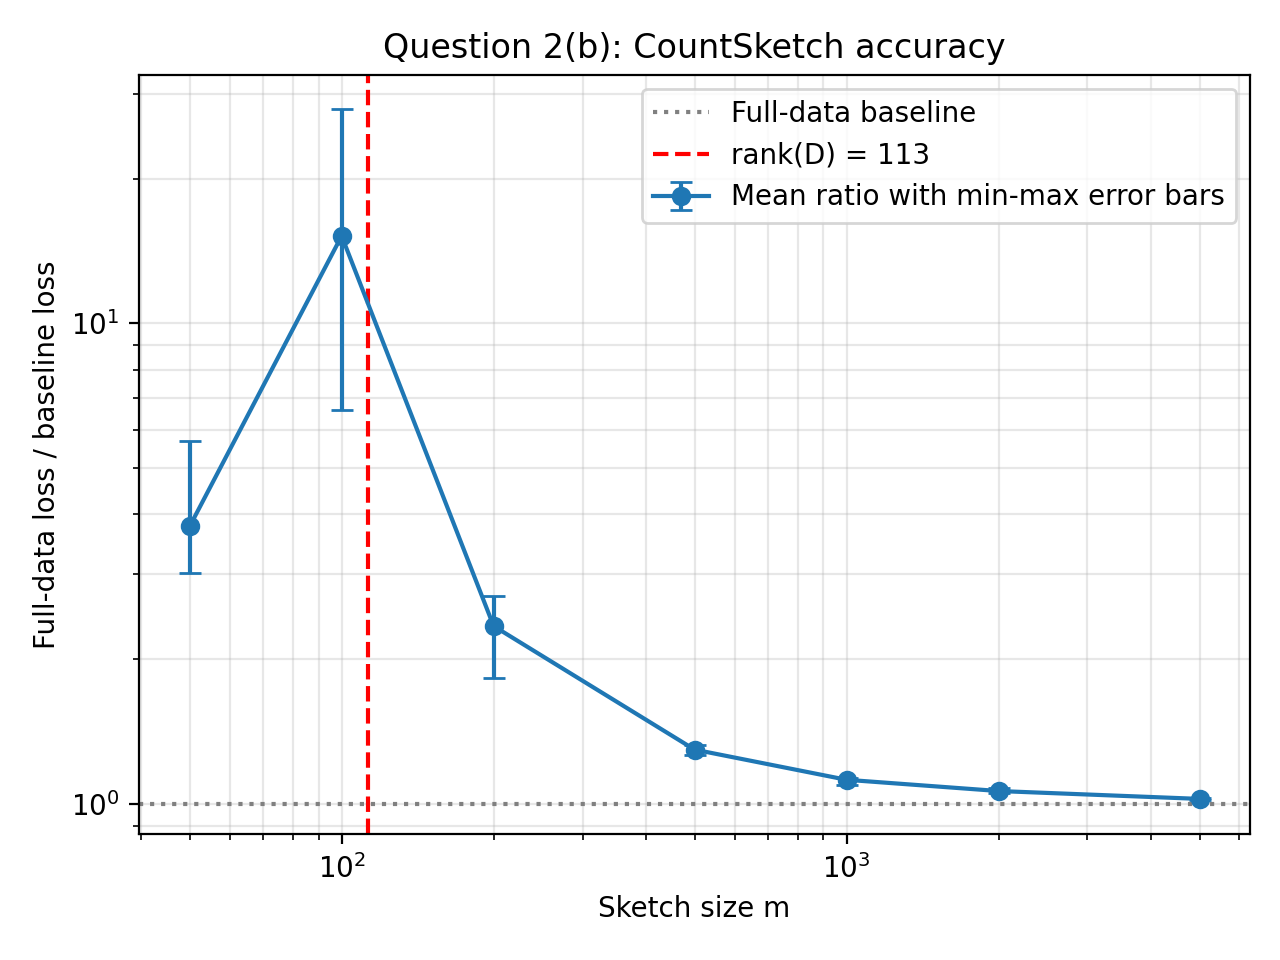
\includegraphics[width=0.78\linewidth]{images/question2_b_ratios.png}
\captionof{figure}{Mean loss ratio on log--log axes, with minimum-to-maximum
error bars. The vertical line marks $\operatorname{rank}(D)=113$.}
\end{center}
\textbf{Discussion.}
For $m=50$ and $100$, both below the numerical rank, the sketched loss is
approximately zero, but the full-data loss is much larger than the optimum.
An underdetermined sketch may interpolate its target without fitting all
original rows well.

The mean ratio rises from $3.7744$ to $15.1856$ near the rank boundary, so the
observed relationship is not monotonic at small $m$. Near-rank sketches can
be unstable; the large range at $m=100$ also shows substantial trial variability.
Above the rank, the mean ratio falls from $2.3413$ at $m=200$ to $1.0229$ at
$m=5000$. The sketched loss becomes nonzero and approaches the baseline loss
as $m$ increases. Since $b$ minimises the full-data loss, $R\geq1$ in exact
arithmetic; every measured ratio satisfies this. Individual trials are in
Appendix A.

\clearpage
\subsection*{(c) Timing comparison}
The same 35 trials as in (b) were timed from before drawing the sketch until
after the sketched least-squares solve. The timing includes bucket/sign
generation, forming $SD$ and $Sy$, and computing $\widetilde a$.
Loss evaluation, output, and plotting are excluded. Speedup is the full-data
solve time divided by the mean sketch-and-solve time.
\begin{center}
\begin{tabular}{rrr}
\toprule
$m$ & Mean time (seconds) & Speedup \\
\midrule
50 & 0.419867 & 5.067 \\
100 & 0.407707 & 5.218 \\
200 & 0.448826 & 4.740 \\
500 & 0.448678 & 4.742 \\
1000 & 0.444807 & 4.783 \\
2000 & 0.429447 & 4.954 \\
5000 & 0.440870 & 4.826 \\
\bottomrule
\end{tabular}
\captionof{table}{Five-trial average timings; full-data baseline: 2.127519 seconds.}
\end{center}
\begin{center}
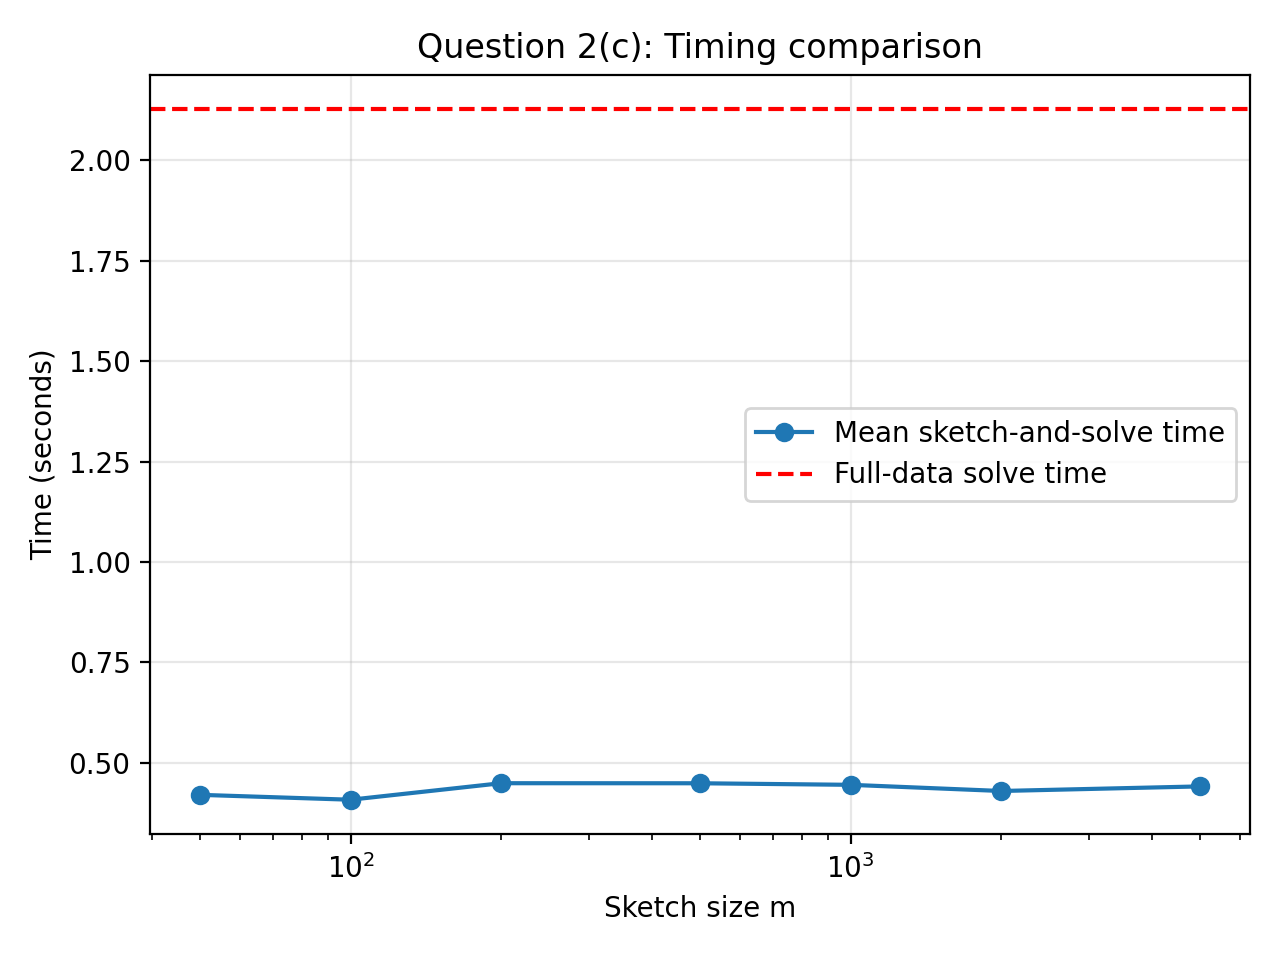
\includegraphics[width=0.90\linewidth]{images/question2_c_times.png}
\captionof{figure}{Mean sketch-and-solve times compared with the full-data solve.}
\end{center}
\textbf{Discussion.}
All sketch sizes are faster than the full-data solve in this run. Their average
times range from $0.4077$ to $0.4488$ seconds, corresponding to approximately
$4.74$--$5.22$ times speedup. There is no clear increasing trend over these
sizes. CountSketch processes the original rows for every $m$, so a substantial
part of its work is shared across sizes; this is consistent with the similar
observed times, although the timing does not isolate the individual operations.
At $m=5000$, the mean loss ratio is only $1.0229$ while the speedup is $4.83$.
These wall-clock measurements describe this execution and can vary between runs.

\clearpage
\subsection*{(d) Residual norm preservation}
The residual of the full solution was calculated once:
\[
 v=Db-y,\qquad \|v\|_2^2=2949.788815.
\]
For each sketch size, 100 independent CountSketches were drawn. Only the
residual vector was sketched; no regression problem was solved again.
For every trial, we recorded $Q=\|Sv\|_2^2/\|v\|_2^2$.
\begin{center}
\begin{tabular}{rrr}
\toprule
$m$ & Mean $Q$ & Sample standard deviation \\
\midrule
50 & 0.987864 & 0.183561 \\
500 & 1.002429 & 0.065296 \\
5000 & 0.998220 & 0.020838 \\
\bottomrule
\end{tabular}
\captionof{table}{Residual squared-norm ratios over 100 trials per size.
Standard deviations use the $N-1$ denominator.}
\end{center}
\begin{center}
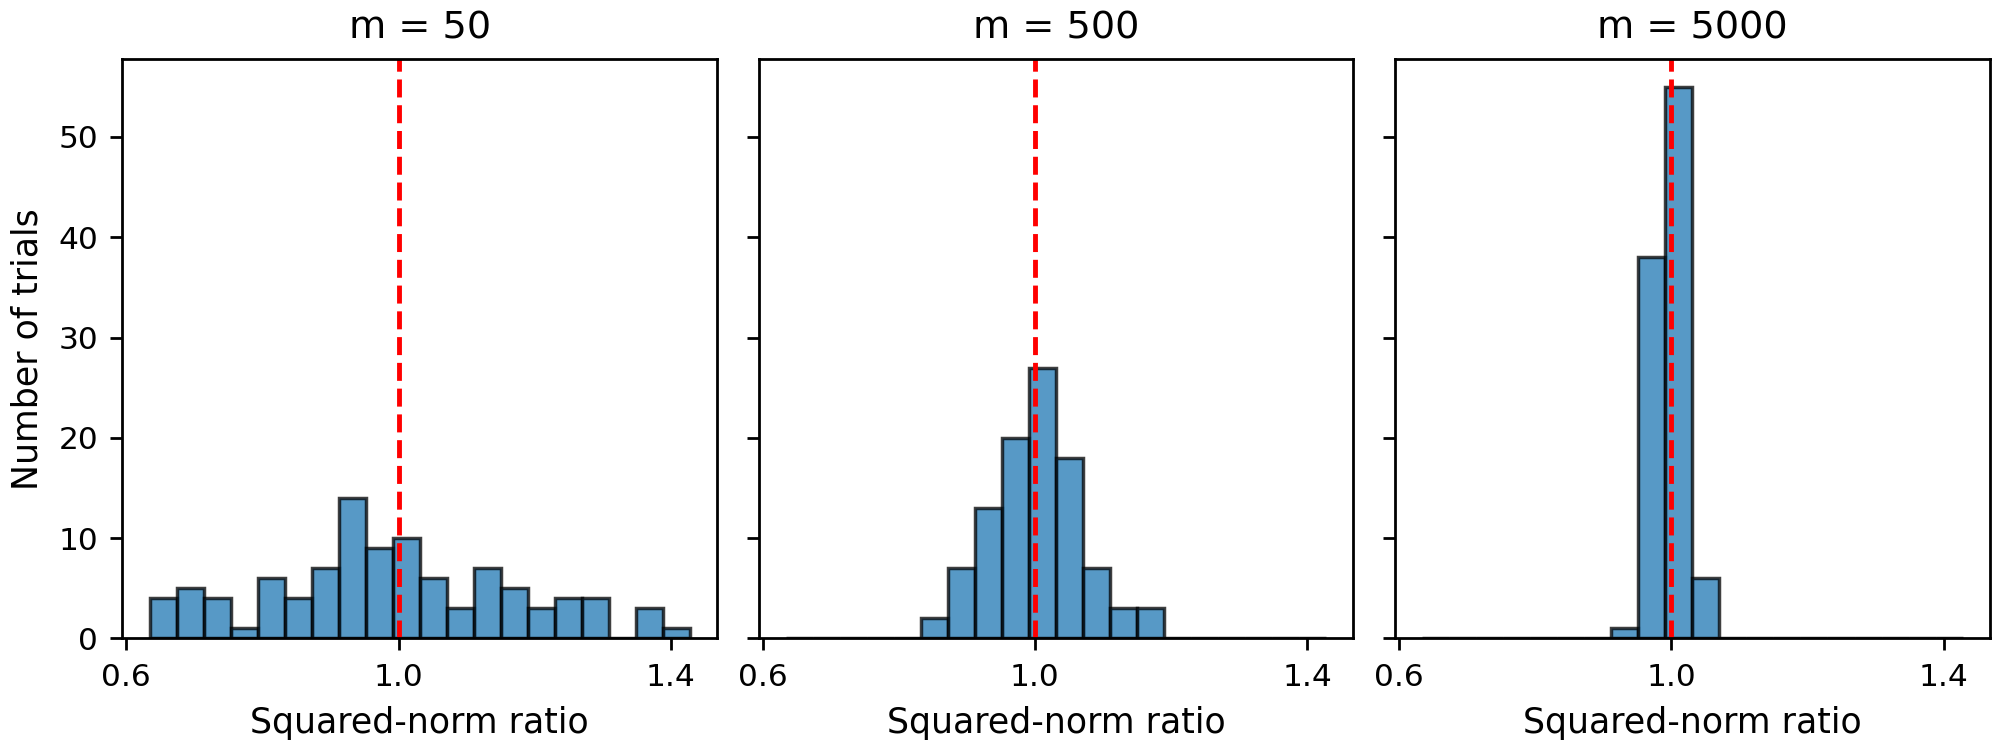
\includegraphics[width=\linewidth]{images/question2_d_histograms.png}
\captionof{figure}{Residual norm-ratio histograms with common bins and axes.}
\end{center}
\textbf{Discussion.}
All three sample means are close to $1$. The spread decreases substantially:
the standard deviation falls from $0.1836$ at $m=50$, to $0.0653$ at $m=500$,
to $0.0208$ at $m=5000$. Thus larger sketches preserve the residual's squared
norm more consistently.

This behaviour follows from the random signs. For a fixed residual, expanding
the sketched squared norm gives
\[
 \|Sv\|_2^2=\sum_i v_i^2+
 2\sum_{i<j}\mathbf 1_{\{h(i)=h(j)\}}\sigma(i)\sigma(j)v_iv_j.
\]
The cross terms have expectation zero, so $\mathbb E[Q]=1$. With independent
uniform buckets and signs,
\[
 \operatorname{Var}(Q)
 =\frac{2}{m}\left(1-
 \frac{\sum_i v_i^4}{(\sum_i v_i^2)^2}\right).
\]
For the same fixed residual, the standard deviation therefore scales as
$1/\sqrt m$. Increasing $m$ by a factor of ten predicts a reduction of
approximately $\sqrt{10}$, consistent with the measured reductions.

\clearpage
\subsection*{(e) CountSketch versus a dense Gaussian sketch}
A single uniformly sampled subset of 50,000 rows was selected without
replacement using seed 123, together with the matching targets.
Both methods and all five repetitions use this exact subset.
The subset baseline was solved separately:
\[
 b'=\arg\min_a\|D'a-y'\|_2^2,\qquad
 \loss(D',y',b')=295.158682.
\]
Both methods use $m=500$. Gaussian entries are independent
$N(0,1/m)$ variables, generated with standard deviation $1/\sqrt{500}$.
The ratio is evaluated on the original subset, using its own baseline.
Only drawing the sketch and forming $SD'$ and $Sy'$ are timed; the solve
and loss evaluation take place after stopping the timer.
\begin{center}
\begin{tabular}{lrr}
\toprule
Method & Mean construction time (s) & Mean loss ratio \\
\midrule
CountSketch & 0.038449 & 3.074398 \\
Gaussian & 0.170562 & 1.263199 \\
\bottomrule
\end{tabular}
\captionof{table}{Five-trial comparison on the same fixed subset.}
\end{center}
\begin{center}
\small
\begin{tabular}{lrrrr}
\toprule
Method & Trial & Time (s) & Subset loss & Loss ratio \\
\midrule
CountSketch & 1 & 0.038466 & 398.945 & 1.351629 \\
CountSketch & 2 & 0.039417 & 393.389 & 1.332804 \\
CountSketch & 3 & 0.038169 & 389.234 & 1.318729 \\
CountSketch & 4 & 0.038080 & 2966.514 & 10.050572 \\
CountSketch & 5 & 0.038117 & 389.095 & 1.318256 \\
Gaussian & 1 & 0.172414 & 390.361 & 1.322545 \\
Gaussian & 2 & 0.173245 & 375.973 & 1.273800 \\
Gaussian & 3 & 0.168305 & 362.918 & 1.229569 \\
Gaussian & 4 & 0.170314 & 373.493 & 1.265397 \\
Gaussian & 5 & 0.168534 & 361.477 & 1.224686 \\
\bottomrule
\end{tabular}
\captionof{table}{Individual trials reveal the unusually large fourth CountSketch loss.}
\end{center}
\textbf{Discussion and choice for the full dataset.}
CountSketch construction is approximately $4.44$ times faster in this
comparison. Gaussian sketches have the smaller average loss ratio
($1.2632$ versus $3.0744$). Four CountSketch trials have ratios between
$1.3183$ and $1.3516$, but trial 4 has ratio $10.0506$ and raises the mean
substantially. This trial is retained in all reported averages.

I would use CountSketch on the full dataset for its construction speed and
memory requirements, while checking the resulting loss and considering a
larger sketch if accuracy is insufficient. A dense Gaussian matrix for
$m=500$ on all 494,021 rows would contain 247,010,500 entries, about
$1.98$ GB in float64 for $S$ alone. CountSketch avoids this dense matrix.
For accuracy at the fixed $m=500$, the Gaussian sketch is the better choice
in these subset experiments; the speed-oriented choice of CountSketch
does not imply that it gave the better loss.

\clearpage
\section*{Appendix A: Individual trials for Question 2(b)}
The full-data baseline loss is 2949.788815. The table reports each
trial's full-data loss, its ratio to that baseline, and its sketched loss.
\begin{center}
\footnotesize
\setlength{\tabcolsep}{10pt}
\begin{tabular}{rrrrr}
\toprule
$m$ & Trial & Full-data loss & Loss ratio & Sketched loss \\
\midrule
50 & 1 & 10002.296 & 3.390852 & $1.306\times10^{-23}$ \\
50 & 2 & 10223.117 & 3.465712 & $9.985\times10^{-24}$ \\
50 & 3 & 9796.732 & 3.321164 & $8.084\times10^{-24}$ \\
50 & 4 & 8890.591 & 3.013975 & $3.033\times10^{-24}$ \\
50 & 5 & 16756.026 & 5.680415 & $3.505\times10^{-23}$ \\
100 & 1 & 30557.870 & 10.359342 & $4.658\times10^{-24}$ \\
100 & 2 & 57980.621 & 19.655855 & $6.777\times10^{-24}$ \\
100 & 3 & 82239.531 & 27.879803 & $1.833\times10^{-23}$ \\
100 & 4 & 33775.820 & 11.450250 & $6.332\times10^{-24}$ \\
100 & 5 & 19417.912 & 6.582814 & $1.539\times10^{-23}$ \\
200 & 1 & 7993.986 & 2.710020 & 1448.856 \\
200 & 2 & 7108.065 & 2.409686 & 1231.782 \\
200 & 3 & 6754.322 & 2.289765 & 1246.702 \\
200 & 4 & 7284.106 & 2.469365 & 1034.153 \\
200 & 5 & 5391.455 & 1.827743 & 1412.200 \\
500 & 1 & 3827.074 & 1.297406 & 2632.984 \\
500 & 2 & 3731.033 & 1.264848 & 1984.387 \\
500 & 3 & 3852.909 & 1.306164 & 2132.465 \\
500 & 4 & 3900.339 & 1.322244 & 2346.513 \\
500 & 5 & 3794.023 & 1.286202 & 2348.737 \\
1000 & 1 & 3293.152 & 1.116402 & 2437.857 \\
1000 & 2 & 3338.988 & 1.131941 & 2589.660 \\
1000 & 3 & 3338.997 & 1.131944 & 2694.533 \\
1000 & 4 & 3229.566 & 1.094846 & 2677.166 \\
1000 & 5 & 3331.915 & 1.129544 & 2724.794 \\
2000 & 1 & 3150.660 & 1.068097 & 2821.299 \\
2000 & 2 & 3175.206 & 1.076418 & 2732.378 \\
2000 & 3 & 3108.708 & 1.053875 & 2849.787 \\
2000 & 4 & 3104.766 & 1.052538 & 2841.355 \\
2000 & 5 & 3126.658 & 1.059960 & 2894.532 \\
5000 & 1 & 3005.386 & 1.018848 & 2844.646 \\
5000 & 2 & 3018.954 & 1.023447 & 2899.033 \\
5000 & 3 & 3017.531 & 1.022965 & 2964.258 \\
5000 & 4 & 3016.756 & 1.022702 & 2895.958 \\
5000 & 5 & 3027.735 & 1.026424 & 2832.304 \\
\bottomrule
\end{tabular}
\end{center}
\subsection*{Reproducibility and saved outputs}
The matrix is reused from \sourcefile{data/D.npy}. The main NumPy generator
uses seed 42 and advances continuously through (b), (d), and (e); each
repetition receives fresh random draws. The subset generator uses seed 123.
Run the full \sourcefile{question2.py} in order to reproduce the draws.
CSV files in \sourcefile{results/} retain all individual measurements for
(b)--(e), including the timings from (c) and the 300 ratios from (d).
The saved baseline coefficients, subset row indices, summaries, three plots,
and \sourcefile{question2_run.log} accompany the results.

\textit{Task source: CSE558 Assignment, data specification on page 1 and
Question 2 on page 3. All numerical tables and figures here are from the
saved local execution; figures summarise the same trials as the tables.}
\end{document}
